\section{Physical problems and applications}

\begin{enumerate}
	\item Obtain the Lagrange's equations of motion of a particle with mass $m$ in a potential $V(r,\theta,\phi)$ in spherical polar coordinates.\\ \setcounter{equation}{0}
	\textbf{Solution}: In spherical polar coordinates, the elementary lengths are $\dd{r}$, $r\dd{\theta}$ and $r\sin{\theta}\dd{\phi}$.
	
	The corresponding velocities are
	\begin{align*}
		v_r=\dv{r}{t}=\dot{r},\quad v_\theta=r\dv{\theta}{t}=r\dot{\theta},\quad v_\phi=r\sin{\theta}\dv{\phi}{t}=r\sin{\theta}\dot{\phi}
	\end{align*}
	
	This gives us the speed of the particle in spherical polar coordinates to be
	\begin{align*}
		v^2&=v_r^2+v_\theta^2+v_\phi^2 \\
		\implies v^2&=\dot{r}^2+r^2\dot{\theta}^2+r^2\sin^2{\theta}\dot{\phi}^2
	\end{align*}
	
	Hence, the kinetic energy of the particle is
	\begin{align*}
		T&=\dfrac{1}{2}mv^2=\dfrac{1}{2}m\qty(\dot{r}^2+r^2\dot{\theta}^2+r^2\sin^2{\theta}\dot{\phi}^2)
	\end{align*}
	
	Assuming that the potential energy is independent of velocities, we can write $V=V(r,\theta,\phi)$. This gives us the Lagrangian to be
	\begin{align}
		\lagrangian&=T-V \nonumber\\
		\implies\lagrangian&=\dfrac{1}{2}m\qty(\dot{r}^2+r^2\dot{\theta}^2+r^2\sin^2{\theta}\dot{\phi}^2)-V(r,\theta,\phi) \label{eqn:lag-spc}
	\end{align}
	
	We choose the generalized coordinates to be the spherical coordinates, i.e. $q_1=r$, $q_2=\theta$ and $q_3=\phi$. The Lagrange's equations of motion are
	\begin{align}
		\dv{t}\pdv{\lagrangian}{\dot{q}_j}-\pdv{\lagrangian}{q_j}&=0,\quad j=1,2,3\label{eqn:eg-1:lagrange-eqn}
	\end{align}
	
	We then obtain the equations of motion in spherical polar coordinates as follows:
	\begin{itemize}
		\item $r$-coordinate:\\
		The Lagrange's equation (\ref{eqn:eg-1:lagrange-eqn}) for $q_1=r$ is
		\begin{align}
			\dv{t}\pdv{\lagrangian}{\dot{q}_1}-\pdv{\lagrangian}{q_1}&=0 \nonumber\\
			\implies\dv{t}\pdv{\lagrangian}{\dot{r}}-\pdv{\lagrangian}{r}&=0 \label{eqn:lag-r-coord}
		\end{align}
		From equation (\ref{eqn:lag-spc}), we have
		\begin{align*}
			\pdv{\lagrangian}{\dot{r}}&=2\times\dfrac{1}{2}m\dot{r}=m\dot{r} \\
			\implies\dv{t}\pdv{\lagrangian}{\dot{r}}&=\dv{t}\qty(m\dot{r})=m\ddot{r}
		\end{align*}
		and also
		\begin{align*}
			\pdv{\lagrangian}{r}&=2\times\dfrac{1}{2}mr\dot{\theta}^2+2\times\dfrac{1}{2}mr\sin^2{\theta}\dot{\phi}^2-\pdv{V}{r} \\
			&=mr\dot{\theta}^2+mr\sin^2{\theta}\dot{\phi}^2-\pdv{V}{r}
		\end{align*}
		Therefore, in equation (\ref{eqn:lag-r-coord}), we obtain
		\begin{align*}
			m\ddot{r}-mr\dot{\theta}^2-mr\sin^2{\theta}\dot{\phi}^2+\pdv{V}{r}&=0 \\
			\implies\Aboxed{m\ddot{r}-mr\qty(\dot{\theta}^2+\sin^2{\theta}\dot{\phi}^2)+\pdv{V}{r}&=0}
		\end{align*}
		
		\item $\theta$-coordinate:\\
		The Lagrange's equation (\ref{eqn:eg-1:lagrange-eqn}) for $q_2=\theta$ is
		\begin{align}
			\dv{t}\pdv{\lagrangian}{\dot{q}_2}-\pdv{\lagrangian}{q_2}&=0 \nonumber\\
			\implies\dv{t}\pdv{\lagrangian}{\dot{\theta}}-\pdv{\lagrangian}{\theta}&=0 \label{eqn:lag-theta-coord}
		\end{align}
		From equation (\ref{eqn:lag-spc}), we have
		\begin{align*}
			\pdv{\lagrangian}{\dot{\theta}}&=2\times\dfrac{1}{2}mr^2\dot{\theta}=mr^2\dot{\theta} \\
			\implies\dv{t}\pdv{\lagrangian}{\dot{\theta}}&=\dv{t}\qty(mr^2\dot{\theta})=mr^2\ddot{\theta}+2mr\dot{r}\dot{\theta}
		\end{align*}
		and also
		\begin{align*}
			\pdv{\lagrangian}{\theta}&=2\times\dfrac{1}{2}mr^2\sin{\theta}\cos{\theta}\dot{\phi}^2-\pdv{V}{\theta} \\
			&=mr^2\sin{\theta}\cos{\theta}\dot{\phi}^2-\pdv{V}{\theta}
		\end{align*}
		Therefore, in equation (\ref{eqn:lag-theta-coord}), we obtain
		\begin{align*}
			\Aboxed{mr^2\ddot{\theta}+2mr\dot{r}\dot{\theta}-mr^2\sin{\theta}\cos{\theta}\dot{\phi}^2+\pdv{V}{\theta}&=0}
		\end{align*}
		
		\item $\phi$-coordinate:\\
		The Lagrange's equation (\ref{eqn:eg-1:lagrange-eqn}) for $q_3=\phi$ is
		\begin{align}
			\dv{t}\pdv{\lagrangian}{\dot{q}_3}-\pdv{\lagrangian}{q_3}&=0 \nonumber\\
			\implies\dv{t}\pdv{\lagrangian}{\dot{\phi}}-\pdv{\lagrangian}{\phi}&=0 \label{eqn:lag-phi-coord}
		\end{align}
		
		From equation (\ref{eqn:lag-spc}), we have
		\begin{align*}
			\pdv{\lagrangian}{\dot{\phi}}&=2\times\dfrac{1}{2}mr^2\sin^2{\theta}\dot{\phi}=mr^2\sin^2{\theta}\dot{\phi} \\
			\implies\dv{t}\pdv{\lagrangian}{\dot{\phi}}&=\dv{t}\qty(mr^2\sin^2{\theta}\dot{\phi})=mr^2\sin^2{\theta}\ddot{\phi}+2mr^2\sin{\theta}\cos{\theta}\dot{\theta}\dot{\phi}+2mr\sin^2{\theta}\dot{r}\dot{\phi}
		\end{align*}
		and also
		\begin{align*}
			\pdv{\lagrangian}{\phi}&=-\pdv{V}{\phi}
		\end{align*}
		
		Therefore, in equation (\ref{eqn:lag-phi-coord}), we obtain
		\begin{align*}
			\Aboxed{mr^2\sin^2{\theta}\ddot{\phi}+2mr^2\sin{\theta}\cos{\theta}\dot{\theta}\dot{\phi}+2mr\sin^2{\theta}\dot{r}\dot{\phi}+\pdv{V}{\phi}&=0}
		\end{align*}
	\end{itemize}
	
	\item Obtain the Lagrange's equations of motion of a particle with mass $m$ in a potential $V(\rho,\phi,z)$ in cylindrical polar coordinates.\\ \setcounter{equation}{0}
	\textbf{Solution}: In cylindrical polar coordinates, the elementary lengths are $\dd{\rho}$, $\rho\dd{\phi}$ and $\dd{z}$.
	
	The corresponding velocities are
	\begin{align*}
		v_\rho=\dv{\rho}{t}=\dot{\rho},\quad v_\phi=\rho\dv{\phi}{t}=\rho\dot{\phi},\quad v_z=\dv{z}{t}=\dot{z}
	\end{align*}
	
	This gives us the speed of the particle in cylindrical polar coordinates to be
	\begin{align*}
		v^2&=v_\rho^2+v_\phi^2+v_z^2 \\
		\implies v^2&=\dot{\rho}^2+\rho^2\dot{\phi}^2+\dot{z}^2
	\end{align*}
	
	Hence, the kinetic energy of the particle is
	\begin{align*}
		T&=\dfrac{1}{2}mv^2=\dfrac{1}{2}m\qty(\dot{\rho}^2+\rho^2\dot{\phi}^2+\dot{z}^2)
	\end{align*}
	
	Assuming that the potential energy is independent of velocities, we can write $V=V(\rho,\phi,z)$. This gives us the Lagrangian to be
	\begin{align}
		\lagrangian&=T-V \nonumber\\
		\implies\lagrangian&=\dfrac{1}{2}m\qty(\dot{\rho}^2+\rho^2\dot{\phi}^2+\dot{z}^2)-V(\rho,\phi,z) \label{eqn:lag-cpc}
	\end{align}
	
	We choose the generalized coordinates to be the cylindrical coordinates, i.e. $q_1=\rho$, $q_2=\phi$ and $q_3=z$. The Lagrange's equations of motion are
	\begin{align}
		\dv{t}\pdv{\lagrangian}{\dot{q}_j}-\pdv{\lagrangian}{q_j}&=0,\quad j=1,2,3\label{eqn:eg-2:lagrange-eqn}
	\end{align}
	
	We then obtain the equations of motion in cylindrical polar coordinates as follows:
	\begin{itemize}
		\item $\rho$-coordinate:\\
		The Lagrange's equation (\ref{eqn:eg-2:lagrange-eqn}) for $q_1=\rho$ is
		\begin{align}
			\dv{t}\pdv{\lagrangian}{\dot{q}_1}-\pdv{\lagrangian}{q_1}&=0 \nonumber\\
			\implies\dv{t}\pdv{\lagrangian}{\dot{\rho}}-\pdv{\lagrangian}{\rho}&=0 \label{eqn:lag-rho-coord}
		\end{align}
		From equation (\ref{eqn:lag-cpc}), we have
		\begin{align*}
			\pdv{\lagrangian}{\dot{\rho}}&=2\times\dfrac{1}{2}m\dot{\rho}=m\dot{\rho} \\
			\implies\dv{t}\pdv{\lagrangian}{\dot{\rho}}&=\dv{t}\qty(m\dot{\rho})=m\ddot{\rho}
		\end{align*}
		and also
		\begin{align*}
			\pdv{\lagrangian}{\rho}&=2\times\dfrac{1}{2}m\rho\dot{\phi}^2-\pdv{V}{\rho} \\
			&=m\rho\dot{\phi}^2-\pdv{V}{\rho}
		\end{align*}
		
		Therefore, in equation (\ref{eqn:lag-rho-coord}), we obtain
		\begin{align*}
			\Aboxed{m\ddot{\rho}-m\rho\dot{\phi}^2+\pdv{V}{\rho}&=0}
		\end{align*}
		
		\item $\phi$-coordinate:\\
		The Lagrange's equation (\ref{eqn:eg-2:lagrange-eqn}) for $q_2=\phi$ is
		\begin{align}
			\dv{t}\pdv{\lagrangian}{\dot{q}_2}-\pdv{\lagrangian}{q_2}&=0 \nonumber\\
			\implies\dv{t}\pdv{\lagrangian}{\dot{\phi}}-\pdv{\lagrangian}{\phi}&=0 \label{eqn:lag-phi-cpc-coord}
		\end{align}
		From equation (\ref{eqn:lag-cpc}), we have
		\begin{align*}
			\pdv{\lagrangian}{\dot{\phi}}&=2\times\dfrac{1}{2}m\rho^2\dot{\phi}=m\rho^2\dot{\phi} \\
			\implies\dv{t}\pdv{\lagrangian}{\dot{\phi}}&=\dv{t}\qty(m\rho^2\dot{\phi})=m\rho^2\ddot{\phi}+2m\rho\dot{\rho}\dot{\phi}
		\end{align*}
		and also
		\begin{align*}
			\pdv{\lagrangian}{\phi}&=-\pdv{V}{\phi}
		\end{align*}
		
		Therefore, in equation (\ref{eqn:lag-phi-cpc-coord}), we obtain
		\begin{align*}
			\Aboxed{m\rho^2\ddot{\phi}+2m\rho\dot{\rho}\dot{\phi}+\pdv{V}{\phi}&=0}
		\end{align*}
		
		\item $z$-coordinate:\\
		The Lagrange's equation (\ref{eqn:eg-2:lagrange-eqn}) for $q_3=z$ is
		\begin{align}
			\dv{t}\pdv{\lagrangian}{\dot{q}_3}-\pdv{\lagrangian}{q_3}&=0 \nonumber\\
			\implies\dv{t}\pdv{\lagrangian}{\dot{z}}-\pdv{\lagrangian}{z}&=0 \label{eqn:lag-z-coord}
		\end{align}
		From equation (\ref{eqn:lag-cpc}), we have
		\begin{align*}
			\pdv{\lagrangian}{\dot{z}}&=2\times\dfrac{1}{2}m\dot{z}=m\dot{z} \\
			\implies\dv{t}\pdv{\lagrangian}{\dot{z}}&=m\ddot{z}
		\end{align*}
		and also
		\begin{align*}
			\pdv{\lagrangian}{z}&=-\pdv{V}{z}
		\end{align*}
		
		Therefore, in equation (\ref{eqn:lag-z-coord}), we obtain
		\begin{align*}
			\Aboxed{m\ddot{z}+\pdv{V}{z}&=0}
		\end{align*}
	\end{itemize}
	
	\newpage
	\item Find the Lagrange's equations of motion of the bob of a simple pendulum.\\ \setcounter{equation}{0}
	\textbf{Solution}:
	\begin{figure}[h!]
		\centering
		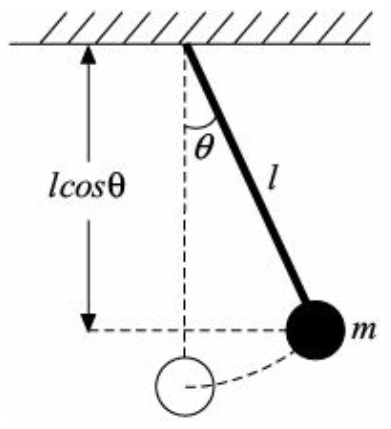
\includegraphics[width=0.25\textwidth]{figures/fig_simple-pendulum-lagrangian.png}
	\end{figure}
	
	Consider a pendulum with a bob of mass $m$, suspended from a fixed ceiling with a massless string of length $l$. Here the number of particles in the system is $N=1$.
	
	The motion of the bob has the following constraints:
	\begin{enumerate}
		\item The bob is free to perform oscillations in a plane only, say the $xy$-plane, and hence
		$$z=0$$
		\item The bob is always at a distance $l$ from the point of suspension, and hence
		$$x^2+y^2=l^2$$
	\end{enumerate}
	Hence, the number of constraints is $k=2$, which gives the degrees of freedom to be $n=3N-k=3\times 1-2=1$. Therefore, the required number of generalized coordinates is also 1.
	
	We can choose the generalized coordinate $q_1=\theta$, where $\theta$ is the angle made by the pendulum string with the vertical axis.
	
	Then the generalized velocity $\dot{\theta}$ would be the angular velocity of the bob about the point of suspension. Hence, the speed of the bob at any instant is
	$$v=l\dot{\theta}$$
	
	This gives the kinetic energy of the bob to be
	\begin{align*}
		T=\dfrac{1}{2}mv^2=\dfrac{1}{2}ml^2\dot{\theta}^2
	\end{align*}
	
	The height of the bob above the lowest point is
	\begin{align*}
		h=l-l\cos{\theta}=l\qty(1-\cos{\theta})
	\end{align*}
	
	So the potential energy of the bob due to gravity is
	\begin{align*}
		V=mgh=mgl(1-\cos{\theta})
	\end{align*}
	
	We obtain the Lagrangian of the system as
	\begin{align}
		\lagrangian&=T-V \nonumber\\
		\implies\lagrangian&=\dfrac{1}{2}ml^2\dot{\theta}^2-mgl(1-\cos{\theta}) \label{eqn:lagrangian:simple-pendulum}
	\end{align}
	Then, the Lagrange's equation for the simple pendulum is
	\begin{align}
		\dv{t}\pdv{\lagrangian}{\dot{q}_1}-\pdv{\lagrangian}{q_1}&=0 \nonumber\\
		\implies\dv{t}\pdv{\lagrangian}{\dot{\theta}}-\pdv{\lagrangian}{\theta}&=0 \label{eqn:lag-equation:simple-pendulum}
	\end{align}
	
	From equation (\ref{eqn:lagrangian:simple-pendulum}), we obtain\vspace{-5ex}
	\begin{multicols}{2}
		
		\begin{align*}
			\pdv{\lagrangian}{\dot{\theta}}&=2\times\dfrac{1}{2}ml^2\dot{\theta}=ml^2\dot{\theta} \\
			\implies\dv{t}\pdv{\lagrangian}{\dot{\theta}}&=ml^2\ddot{\theta}
		\end{align*}
		
		\begin{align*}
			\pdv{\lagrangian}{\theta}&=\pdv{\theta}\qty[-mgl(1-\cos{\theta})] \\
			&=\pdv{\theta}\qty[-mgl+mgl\cos{\theta}] \\
			&=-mgl\sin{\theta}
		\end{align*}
		
	\end{multicols}
	
	Substituting in equation (\ref{eqn:lag-equation:simple-pendulum}), we obtain
	\begin{align}
		ml^2\ddot{\theta}+mgl\sin{\theta}&=0 \nonumber\\
		\implies \ddot{\theta}+\qty(\dfrac{g}{l})\sin{\theta}&=0 \label{eqn:equation-motion:simple-pendulum}
	\end{align}
	Equation (\ref{eqn:equation-motion:simple-pendulum}) is the equation of motion for the bob of the simple pendulum.
	
	For small oscillations, we can consider $\theta$ to be small and so we can use the small-angle approximation, i.e.
	$$\sin{\theta}\approx\theta$$
	
	Then equation (\ref{eqn:equation-motion:simple-pendulum}) becomes as follows:
	\begin{align}
		\ddot{\theta}+\qty(\dfrac{g}{l})\theta&=0 \nonumber\\
		\implies\dv[2]{\theta}{t}&=-\qty(\dfrac{g}{l})\theta \label{eqn:equation-motion-approx:simple-pendulum}
	\end{align}
	Comparing equation (\ref{eqn:equation-motion-approx:simple-pendulum}) with the ODE for simple harmonic motion (SHM), i.e.
	\begin{align*}
		\dv[2]{y}{t}&=-\omega^2y
	\end{align*}
	we find that the pendulum bob also performs SHM with an angular frequency
	\begin{align*}
		\omega^2&=\dfrac{g}{l} \\
		\implies\omega&=\sqrt{\dfrac{g}{l}}
	\end{align*}
	
	The time period of the simple pendulum is
	\begin{align*}
		T&=\dfrac{2\pi}{\omega} \\
		\implies T&=2\pi\sqrt{\dfrac{l}{g}}
	\end{align*}
	
	\newpage
	\item A rigid body capable of oscillating in a vertical plane about a fixed horizontal axis is called a compound pendulum.
	\begin{enumerate}[(i)]
		\item Set up its Lagrangian.
		\item Obtain its equations of motion.
		\item Find the time period of the pendulum.
	\end{enumerate} \setcounter{equation}{0}
	\textbf{Solution}:
	\begin{figure}[h!]
		\centering
		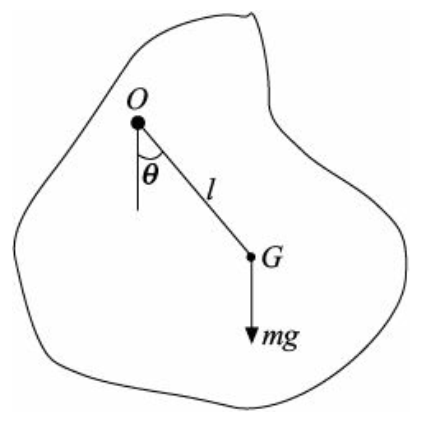
\includegraphics[width=0.3\textwidth]{figures/fig_compound-pendulum-lagrangian.png}
	\end{figure}
	Let us consider a rigid body that is fixed at point $O$, through which the axis of oscillations passes. Let $m$ be its mass, $G$ its centre of mass which is at a distance $l$ from $O$ and $I$ its moment of inertia about the axis of oscillation.
	
	Because the body is rigid, the separation between any two arbitrary points in the body always remains constant. Hence, knowing the coordinates of any single point is sufficient to completely describe the motion of the entire body. So we consider the particle located at the centre of gravity $G$ to be representative of the entire body.
	
	Therefore, similar to the case of the simple pendulum, the degrees of freedom is 1, and we can choose the generalized coordinate $q_1=\theta$, where $\theta$ is the angle made by the line $OG$ with the vertical axis.
	
	The rotational kinetic energy of the body is
	\begin{align*}
		T=\dfrac{1}{2}I\dot{\theta}^2
	\end{align*}
	
	With respect to the point of oscillation, the potential energy of the rigid body is
	\begin{align*}
		V=-mgl\cos{\theta}
	\end{align*}
	
	Therefore, the Lagrangian of the compound pendulum is
	\begin{align}
		\lagrangian&=T-V \nonumber\\
		\implies\lagrangian&=\dfrac{1}{2}I\dot{\theta}^2+mgl\cos{\theta} \label{eqn:lagrangian:compound-pendulum}
	\end{align}
	
	Then, the Lagrange's equation for the compound pendulum is
	\begin{align}
		\dv{t}\pdv{\lagrangian}{\dot{q}_1}-\pdv{\lagrangian}{q_1}&=0 \nonumber\\
		\implies\dv{t}\pdv{\lagrangian}{\dot{\theta}}-\pdv{\lagrangian}{\theta}&=0 \label{eqn:lag-equation:compound-pendulum}
	\end{align}
	
	\newpage
	From equation (\ref{eqn:lagrangian:compound-pendulum}), we obtain\vspace{-5ex}
	\begin{multicols}{2}
		
		\begin{align*}
			\pdv{\lagrangian}{\dot{\theta}}&=2\times\dfrac{1}{2}I\dot{\theta}=I\dot{\theta} \\
			\implies\dv{t}\pdv{\lagrangian}{\dot{\theta}}&=I\ddot{\theta}
		\end{align*}
		
		\begin{align*}
			\pdv{\lagrangian}{\theta}&=\pdv{\theta}\qty[mgl\cos{\theta}] \\
			&=-mgl\sin{\theta}
		\end{align*}
		
	\end{multicols}
	
	Substituting in equation (\ref{eqn:lag-equation:compound-pendulum}), we obtain
	\begin{align}
		I\ddot{\theta}+mgl\sin{\theta}&=0 \nonumber\\
		\implies\ddot{\theta}+\qty(\dfrac{mgl}{I})\sin{\theta}&=0 \label{eqn:equation-motion:compound-pendulum} 
	\end{align}
	Equation (\ref{eqn:equation-motion:compound-pendulum}) is the equation of motion for the compound pendulum.
	
	Using the small-angle oscillations, we have $\sin{\theta}\approx\theta$. Then equation (\ref{eqn:equation-motion:compound-pendulum}) becomes as follows:
	\begin{align}
		\ddot{\theta}&=-\qty(\dfrac{mgl}{I})\theta \nonumber\\
		\implies\dv[2]{\theta}{t}&=-\qty(\dfrac{mgl}{I})\theta \label{eqn:equation-motion-approx:compound-pendulum}
	\end{align}
	Comparing equation (\ref{eqn:equation-motion-approx:compound-pendulum}) with the ODE for simple harmonic motion (SHM), i.e.
	\begin{align*}
		\dv[2]{y}{t}&=-\omega^2y
	\end{align*}
	we find that the compound pendulum also performs SHM with an angular frequency
	\begin{align*}
		\omega^2&=\dfrac{mgl}{I} \\
		\implies\omega&=\sqrt{\dfrac{mgl}{I}}
	\end{align*}
	
	The time period of the compound pendulum is
	\begin{align*}
		T&=\dfrac{2\pi}{\omega} \\
		\implies T&=2\pi\sqrt{\dfrac{I}{mgl}}
	\end{align*}
	If $k$ is the radius of gyration of the compound pendulum, then we have $I=m(k^2+l^2)$. Then the time period of the compound pendulum becomes
	\begin{align*}
		T&=2\pi\sqrt{\dfrac{m(k^2+l^2)}{mgl}} \\
		\implies T&=2\pi\sqrt{\dfrac{k^2+l^2}{gl}}
	\end{align*}
\end{enumerate}